\documentclass[a4paper,11pt, footsepline]{book}
\usepackage[T1]{fontenc}
\usepackage[utf8]{inputenc}
\usepackage{lmodern}

\usepackage{hyperref}
\usepackage{graphicx}
\usepackage[english]{babel}

\usepackage{graphicx}
\usepackage{amsmath}
\usepackage{nameref}
\usepackage{hyperref}
\usepackage[linesnumbered, boxed]{algorithm2e}
\usepackage[automark,footsepline,plainfootsepline,headsepline]{scrpage2}

\SetAlCapSkip{1em}

\SetKwInput{KwInput}{Input}
\SetKwInput{KwOutput}{Output}

\usepackage[printonlyused]{acronym}

\newcommand*{\fullref}[1]{\hyperref[{#1}]{\autoref*{#1} \nameref*{#1}}} % One single link
\renewcommand*\footnoterule{}

\makeatletter
\renewcommand{\@chapapp}{}% Not necessary...
\newenvironment{chapquote}[2][2em]
  {\setlength{\@tempdima}{#1}%
   \def\chapquote@author{#2}%
   \parshape 1 \@tempdima \dimexpr\textwidth-2\@tempdima\relax%
   \itshape}
  {\par\normalfont\hfill--\ \chapquote@author\hspace*{\@tempdima}\par\bigskip}
\makeatother




% Book's title and subtitle
\title{\Huge \textbf{High Performance Computing with Python} \vspace{4mm} \\ \huge Final Report}
% Author
% \author{\textsc{First-name Last-name}\footnote{email address}}
\author{\textsc{Name} \\ \vspace{3mm}\text{matricular number}  \\
\vspace{3mm}\text{mail}}


\begin{document}

\makeatletter
    \begin{titlepage}
        \begin{center}
            
\includegraphics[width=0.5\linewidth]{logos/Uni_Logo-Grundversion_E1_A4_CMYK.eps}\\[4ex]
            {\huge \bfseries  \@title }\\[2ex] 
            {\LARGE  \@author}\\[30ex] 
            {\large \@date}
        \end{center}
    \end{titlepage}
\makeatother
\thispagestyle{empty}
\newpage



\tableofcontents

\begin{acronym}
\section*{Abbreviations}
\acro{bte}[BTE]{Boltzman Transport Equation}
\acro{ci}[CI]{Continuous Integration}
\acro{lbm}[LBM]{Lattice Boltzman Method}
\end{acronym}
\mainmatter

\chapter{Introduction}
\cite{timm2016lattice}

The \acf{lbm} is a numerical parallelizable and efficient scheme for simulating fluid flows. In addition, the \ac{lbm} can be extended with boundary conditions. The key property of the \ac{lbm} is that it is a discrete kinetic theory approach featuring a mescoscale description of the microstructure of the fluid instead of discretising macroscopic continuum equations. Other key advantages of the \ac{lbm} include: efficient implementation by parallelization.

All code is available at \url{https://github.com/infomon/lattice_boltzman_parallel_solver} under BSD license. We give the instructions how to reproduce the results of the experiments conducted in this report in the \textit{README}.

\section*{Structure of report}
The remainder of the report is organized as follows:
\begin{itemize}
\item \textbf{Chapter \ref{ch-method}} describes the \ac{lbm}. More specifically, we describe how we discretize the \textit{Boltzman transport equation} resulting in the \ac{lbm}. We also show how macroscopic quantities, e.g. density and velocity, can be calculated from the microscopic simulation. In addition, we describe several boundary conditions that can be applied in the \ac{lbm}.
\item \textbf{Chapter \ref{ch-implementation}} describes how the \ac{lbm} is implemented using \textit{Python} as programming language. We also show how we parallelized the implementation and how we ensured software quality by unit testing.
\item \textbf{Chapter \ref{ch-results}} conducts extensive experiments showing the applicability and correctness of the implementation of the solver for the \ac{lbm}. 
\item \textbf{Chapter \ref{ch-conclusion}} concludes this report.
\end{itemize}
\chapter{Lattice boltzman method}\label{ch-method}
\section{Overview}
In this chapter we describe the \acf{lbm}. The basic idea of the \ac{lbm} is to statistically consider particles and consider them as a whole unit.
\section{\acf{bte}}\label{sec-bte}
The boltzman transport equation defines the fundamental differential equation of kinematic gas theory.
\subsection*{Streaming}
\subsection*{Collisions}
\subsection*{Discretization of the \ac{bte}}
\begin{figure}[h!]
  \begin{center}
   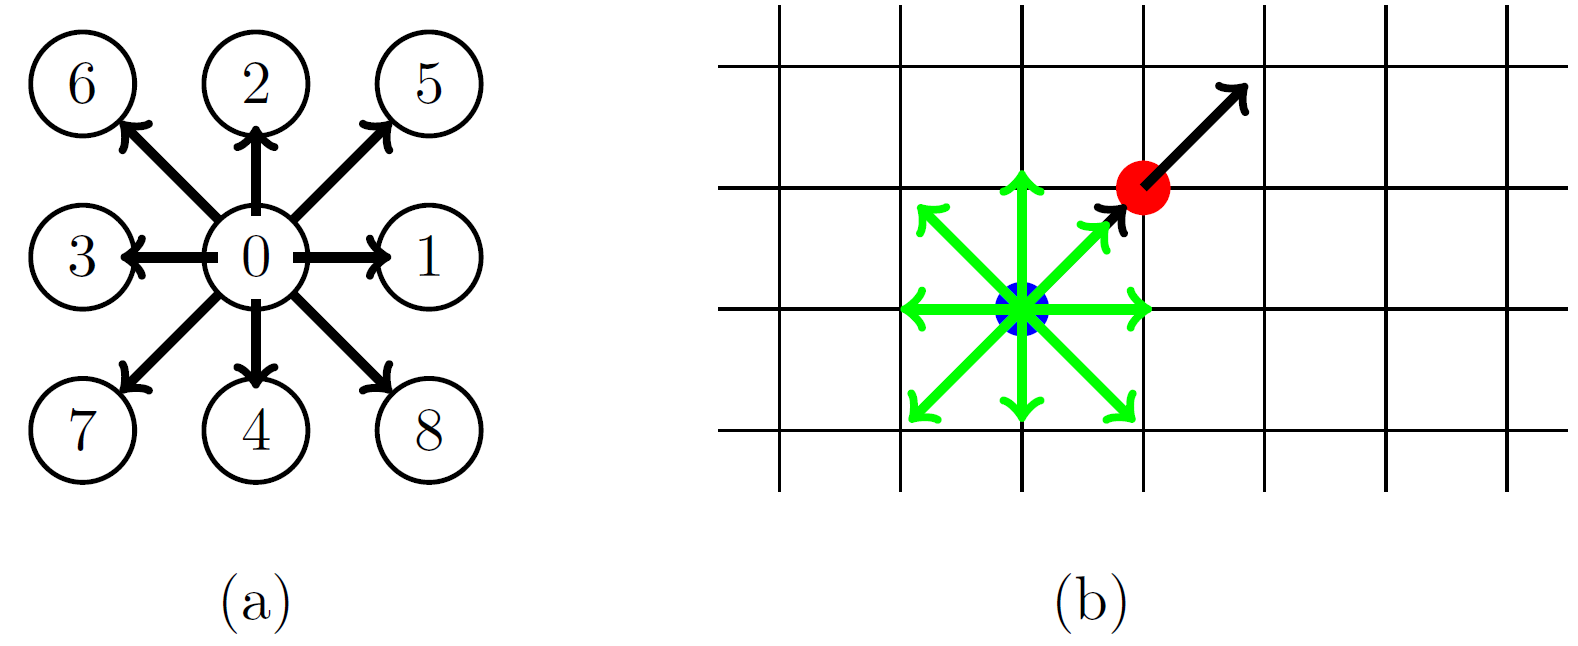
\includegraphics[width=10cm]{logos/Gitter_LBM.png}
   \caption{example figure}
  \label{fig:mesh}
  \end{center}
\end{figure}
\section{Lattice}
\section{Moment update}\label{sec-momentUpdate}
In the \ac{lbm}, the density $\rho$ and velocity $\mathbf{u}$ are defined by the zeroth and first moments of the probability distribution function $f_i$, respectively:
\begin{align*} 
\rho(\mathbf{x},t) &=  \int f(\mathbf{x}, \mathbf{u},t)~d^{3}\mathbf{u}, \\ 
\mathbf{u}(\mathbf{x},t) &=  \frac{1}{\rho(\mathbf{x})}\int f(\mathbf{x}, \mathbf{u},t)\cdot\mathbf{c}(\mathbf{u})~d^{3}\mathbf{u}.
\end{align*}
Discretizing those equation we get
\begin{align*} 
\rho(\mathbf{x}) &=  \sum\limits_{i} f_{i}, \\ 
\mathbf{u}(\mathbf{x}) &=  \sum\limits_{i} f_{i}\mathbf{c}_{i}.
\end{align*}
\section{Boundary conditions}\label{sec-boundaryConditions}
One key advantage of the \ac{lbm} is its easy implementation of boundary conditions. To apply boundary conditions the distributions function $f_i$ is modified at each boundary lattice point $\mathbf{x}_{b}$ in each time step. That is $f_i(\mathbf{x}_{b}+c_{i}\Delta t, t+\Delta t)=f_{i}^{\ast}(\mathbf{x}_b,t)$, where $\mathbf{x}_b$ denotes the boundary nodes, $f_{i}^{\ast}$ the distribution function before the streaming and $f_{i}$ the distribution function after the streaming.

One question that arises is where the boundary nodes $\mathbf{x}_b$ are defined. We distinguish between so called \textit{wet nodes} and \textit{dry nodes} due to different domains, i.e. computational and physical domain. In the former, the computation and physical domain is the same (i.e. the boundaries are placed on the lattice nodes) but this comes with a increased difficulty for the implementation. In the latter the physical domain is half a cell away from the computational domain (i.e. the boundaries are located between the lattice nodes) retaining second order accuracy as long as the boundary is placed exactly in the middle of the lattice nodes.

Below we describe several boundary conditions. Note, that they can be arbitrarily combined as long as they do not contradict themselves.
\subsection*{Periodic}
For a periodic boundary condition the flow leaving a boundary re-enters the domain on the opposite side of the domain. Note, that this boundary condition does not simulate reality. This is that $f_{i}(\mathbf{x}_{1},t)=f_{i}(\mathbf{x}_{N},t)$, where $\mathbf{x}_{1}$ and $\mathbf{x}_{N}$ are the first and last node in the physical domain, respectively. Visually, we can imagine that we have a cylindrical shape.
The periodic boundary condition is implicitly implemented by the streaming function.
\subsection*{Bounce-back}
The bounce-back boundary condition applies a no-slip condition at the boundary. It simulates the interaction between the fluid with a non-moving wall without slip. It can also be applied to a stationary obstacle such as a plate.
\subsection*{Moving wall}
\subsection*{Inlet}
\subsection*{Outlet}
\subsection*{Periodic with pressure variation}
\chapter{Implementation}\label{ch-implementation}
In this chapter we will describe how we implement the algorithm using \textit{Python} as programming language.
\section{Overview}
Algo. \ref{algo-pseudeocode} shows the pseudocode of the iteration loop of the \ac{lbm}. As input we can specify the geometry of the physical domain, the boundary conditions (see section \ref{sec-boundaryConditions} for more details) as well as the initial conditions. 

First we initialize the density $\rho$ and velocity $\mathbf{u}$ and compute the initial value of the probability density function $f_{i}^{eq}=f_{i}$. 

Then we iterate in a loop over several steps as long as the stopping criterion (e.g. maximum time steps) is not satisfied. Note, that there is some flexibility when to apply which step. The following order of steps corresponds to the order in the implementation of the \ac{lbm}. We first compute the equilibrium function $f_{i}^{eq}$ given the current density $\rho$ and velocity $\mathbf{u}$. In the collision step we simulate the effects of collisions between particles (see section \ref{sec-bte} for more details). After that, we simulate the streaming of $f_i$, i.e. we simulate the movement of particles to the nearest neighbour lattice nodes using the D2Q9 discretization. Then we apply potential boundary conditions on the probability density function $f_i$. Lastly, we compute the density $\rho$ and velocity $\mathbf{u}$ (see section \ref{sec-momentUpdate} for details on the formulas on how to compute the macroscopic quantities).

After running the \ac{lbm} we can obtain the density $\rho$ and velocity $\mathbf{u}$ as macroscopic quantities.

\begin{algorithm} %or another one check
 \caption{\label{algo-pseudeocode}Pseudocode of the iteration loop of the \ac{lbm}.}
     \SetAlgoLined
     \KwInput{Geometry and parameters $l$, $h$, $U$, $\nu$,...; boundary conditions; initial conditions}
     \KwOutput{Final density $\rho$ and velocity $\mathbf{u}$}
     initialize $\rho$ and $\mathbf{u}$ \\
     compute $f_i$ and $f_i^{eq}$ \\
     \While{stopping criterion is not satisfied}{
      compute equilibrium function $\rho,~\mathbf{u}\rightarrow f_{i}^{eq}$\\
      collision step $f_{i}^{\ast}=f_{i}(\mathbf{x},t)-\frac{\Delta t}{\tau}(f_{i}(\mathbf{x},t)-f_{i}^{eq}(\mathbf{x},t))$ (see section \ref{sec-bte})\\
      streaming $f_{i}(\mathbf{x}+c_{i}\Delta t, t+\Delta t)=f_{i}^{\ast}(\mathbf{x},t)$ (see section \ref{sec-bte})\\
      apply boundary conditions $f_i(\mathbf{x}_{b}+c_{i}\Delta t, t+\Delta t)=f_{i}^{\ast}(\mathbf{x}_b,t)$ (see section \ref{sec-boundaryConditions})\\
      moment update $f_i \rightarrow \rho,~\mathbf{u}$ (see section \ref{sec-momentUpdate})
     }

\end{algorithm}
\section{Parallelization}
\section{Software quality}
\subsection*{Static typing}
Python is a dynamically typed language. That is that the Python interpreter does type checking only in runtime and the type of a variable is allowed to change. The opposite of dynamic typing is static typing. It is introduced by \textit{PEP 484} in Python. In static typing, the types of the variables are checked before runtime and the change of types is generally not allowed. Note, as an exception type casting is a way to change the type of a variable in many languages.

Dynamic typing allows for rapid prototyping and thus it enables fast software development. On the other side static typing can help to catch errors due to type errors, document the code and help to build a cleaner software architecture. The last point in particular ensures that the programmer thinks about the types of the variables and uses the correct types. Thus, in any larger project typing is critical to build and maintain clean code.
\subsection*{Unit testing}
One key component of every software project is extensive testing of the software. To this end, we implement several unit tests in order to validate the expected behavior of the implemented functions. We integrate the unit tests into \ac{ci} using \textit{Travis CI} as build server so that the implementation and its potential unintentional modifications are validated for each commit to the repository.
\chapter{Numerical results}\label{ch-results}
To demonstrate the \ac{lbm} we conduct several experiments with different combinations of boundary conditions.
\section{Shear wave decay}
To validate the implementation, we compare the simulated solutions with analytical solutions.

We choose the following simulation parameters for our experiments about the planar couette flow:
\begin{itemize}
\setlength\itemsep{0.15em}
\item lattice grid shape $=50\times 50$
\item $\omega=1.0$
\item Sinusoidal density in x-direction $\rho(\mathbf{x},0)=\rho_{0}+\epsilon_{\rho}\sin(\frac{2\pi x}{l_x})$
\begin{itemize}
\setlength\itemsep{0.1em}
\item $\rho_{0}(\mathbf{x})=0.5$
\item $\epsilon_{\rho}=0.08$
\item $\mathbf{u}_{initial}(\mathbf{x})=0.0$
\end{itemize}
\item Sinusoidal velocity in y-direction $\mathbf{u}_{x}(\mathbf{x},0)=\epsilon_{\mathbf{u}}\sin(\frac{2\pi y}{l_y})$
\begin{itemize}
\setlength\itemsep{0.1em}
\item $\rho_{initial}(\mathbf{x})=0.0$
\item $\epsilon_{\mathbf{u}}=0.08$
\end{itemize}
\item time steps $=2000$
\end{itemize}
\section{Planar couette flow}
The planar couette flow is a steady, laminar flow between two infinitely long, parallel plates with a fixed distance. One of those plates moves tangentially at a velocity of $U$ relative to the other plate, which itself is stationary. The flow is caused by the viscous drag force acting on the fluid.

We choose the following simulation parameters for our experiments about the planar couette flow:
\begin{itemize}
\setlength\itemsep{0.15em}
\item lattice grid shape $=20\times 30$
\item $\omega=1.0$
\item $U=0.05$
\item $\rho_{initial}(\mathbf{x})=1.0$
\item $\mathbf{u}_{initial}(\mathbf{x})=0.0$
\item time steps $=4000$
\end{itemize}
\section{Planar poiseuille flow}
The planar poiseuille flow is a steady flow between two non-moving plates. The flow is caused by a constant pressure gradient $\frac{dp}{dx}$ in the axial direction, $x$, parallel to two infinitely long parallel plates, seperated by a distance $h$.

We choose the following simulation parameters for our experiments about the planar poiseuille flow:
\begin{itemize}
\setlength\itemsep{0.15em}
\item lattice grid shape $=200\times 30$
\item $\omega=1.5$
\item $p_{out}=\frac{1}{3}$
\item $\Delta p=0.001111$
\item $\rho_{initial}(\mathbf{x})=1.0$
\item $\mathbf{u}_{initial}(\mathbf{x})=0.0$
\item time steps $=5000$
\end{itemize}

Some error can occure due to:
\begin{itemize}
\item Inaccuracy introduced by the bounce-back boundary condition
\end{itemize}
\section{Von K\'{a}rm\'{a}n's vortex street}
\section{Scaling tests}
\chapter{Conclusions}\label{ch-conclusion}


\newpage

\bibliographystyle{unsrt}
\bibliography{biblio}

\end{document}
